\newprob{1715431740}
{
    % active phys p284 15
    小克從離地1 m 高的平台從靜止跳起,其質量為 70 kg。
    \begin{parts}
        \part 估算小克剛着地前的速率。\zzh{2}
        \part \begin{subparts}
            \subpart 小克着地時的動量變化是多少?\zzh{1}
            \subpart 假設小克從剛着地至完全靜止需時 0.1 s。估算小克着地時地面作用在他身 上的平均力。 \zzh{2}
        \end{subparts}
        \part 人們着地時一般會屈膝。舉出着地時屈膝的一個好處。 \zzh{1}
    \end{parts}
    \dlines{1}\clearpage\dlines{1}
}{
    \sol
    \par{\par\centering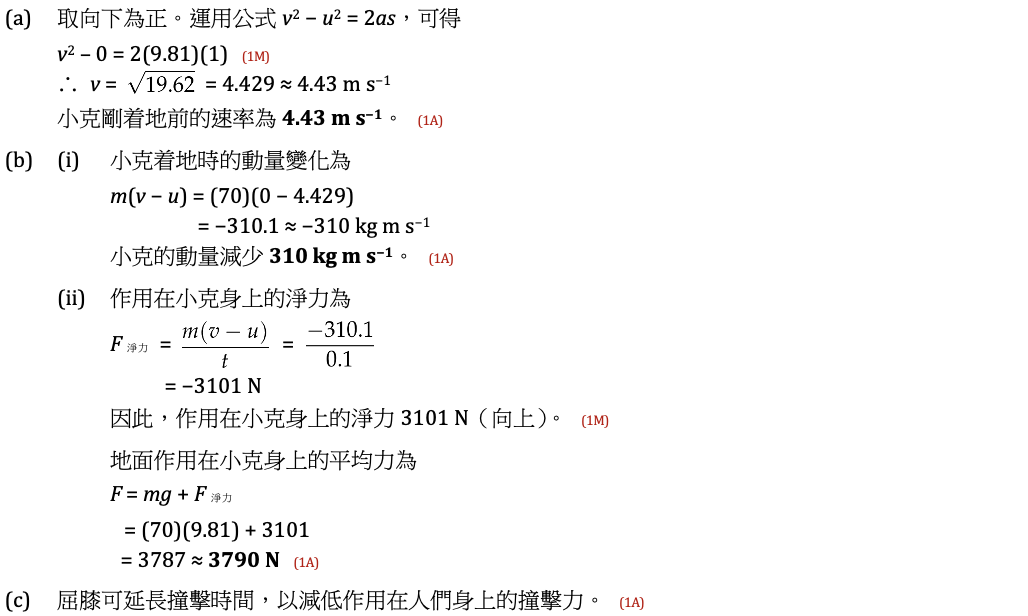
\includegraphics[width=\textwidth]{./img/ch5_momentum_lq_2024-05-11-22-42-41.png}\par}
}

\newprob{1715432376}
{
    % active phys p286 20
    一架直升機停留在空中。直升機的質量為 1200 kg,其葉片長8 m。\bigskip
    \par{\par\centering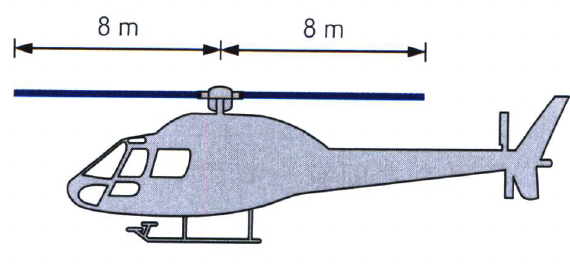
\includegraphics[width=.4\textwidth]{./img/ch5_momentum_lq_2024-05-11-21-00-18.png}\par}\bigskip
    \begin{parts}
        \part 直升機的葉片旋轉時,不斷上方的空氣抽往 下方。試扼要解釋何以直升機能藉此停留在 空中。 \par\zzh{2}
        \part 假設葉片上方的空氣起初靜止。空氣的密度 為 \qty{1.2}{kg.m^{-3}}。
        \begin{subparts}
            \subpart 估算葉片下方空氣的速率。\zzh{3}
            \subpart 估算直升機引擎的功率。\zzh{2}
        \end{subparts}
        \part 葉片必須傾斜,才能使直升機向前推進。假 如直升機水平推進時,葉片與水平成 \dg{5}角, 證明作用在機上的向前推力約為1000 N。試 輔以隔離體圖,解釋你的答案。 \zzh{2}
    \end{parts}
    \dlines{1}\clearpage\dlines{1}
}{
    \sol
    \par{\par\centering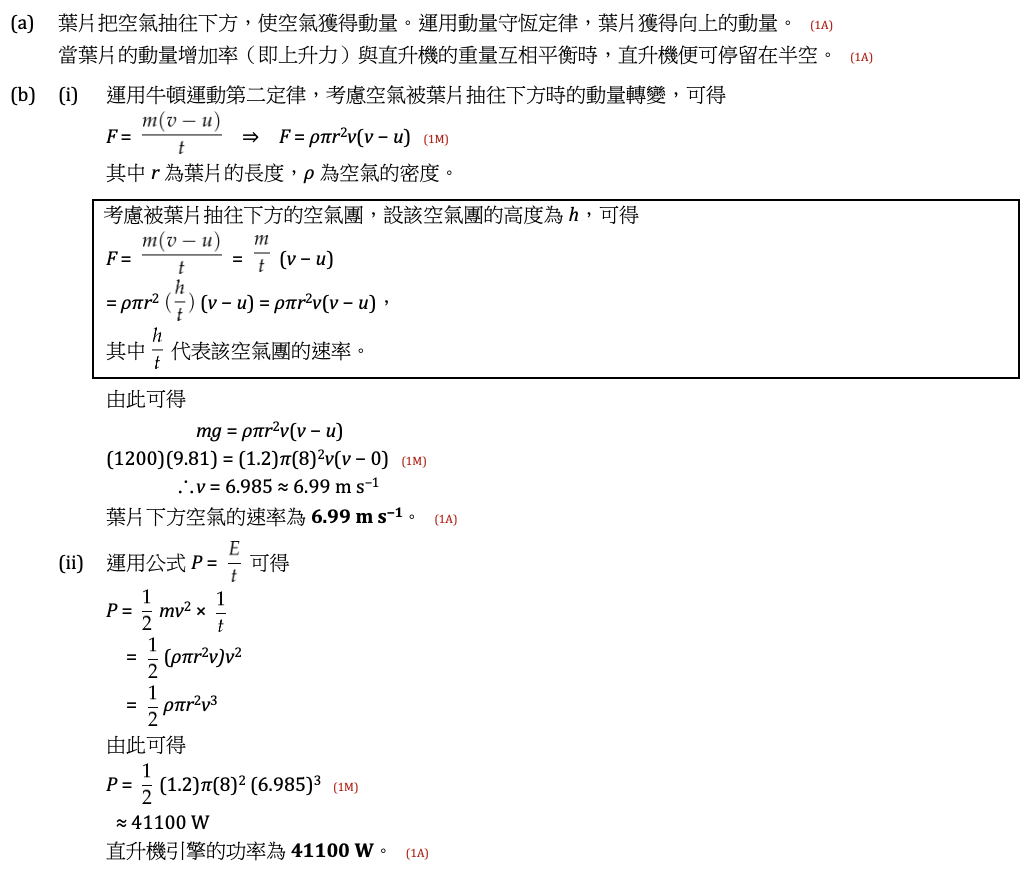
\includegraphics[width=.9\textwidth]{./img/ch5_momentum_lq_2024-05-11-22-43-32.png}\par}
    \par{\par\centering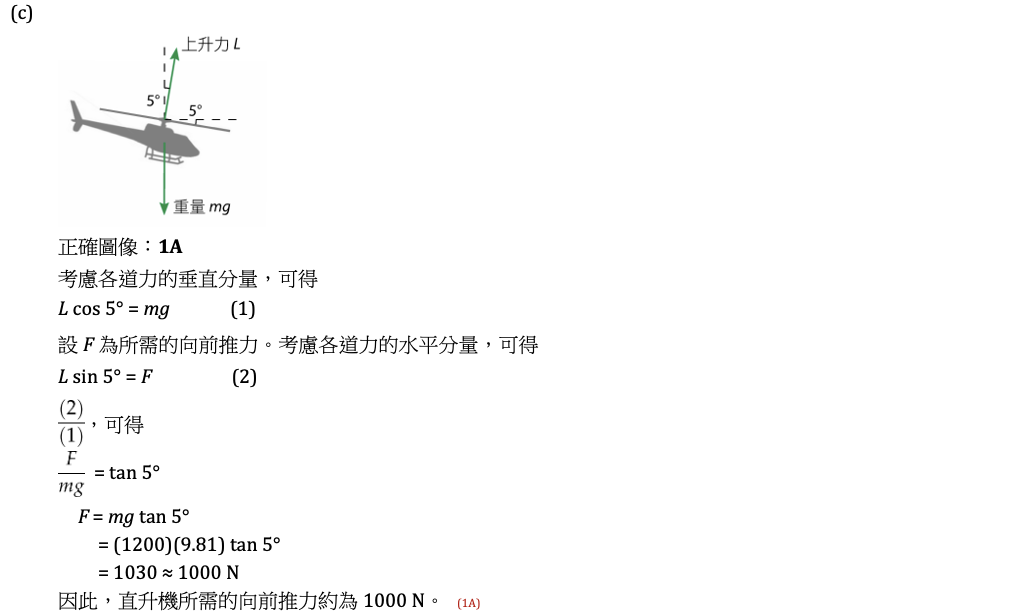
\includegraphics[width=.9\textwidth]{./img/ch5_momentum_lq_2024-05-11-22-43-49.png}\par}
}

\newprob{1715432617}
{
    % active  phys p289 *4
    小球 $A$(質量為$m_A$)與小球$B$(質量為$m_B$)發生 對正彈性碰撞。碰撞前,小球$A$以速率$u$朝着靜 止的小球$B$衝去。碰撞後,$A$、$B$ 兩球分別以速 率$v_A$和$v_B$移動。\bigskip \par{\par\centering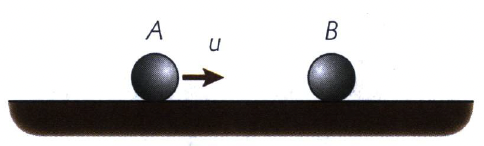
\includegraphics[width=.3\textwidth]{./img/ch5_momentum_lq_2024-05-11-21-04-47.png}\par}\bigskip
    \begin{parts}
        \part 證明$m_A(u-v_A)=m_Bv_B$。\zzh{2}
        \part 證明$m_A(u^2-v_A^2)=m_Bv_B^2$。\zzh{2}
        \part 由此,證明\zzh{3}
        \begin{subparts}
            \subpart $v_A=\dfrac{m_a-m_B}{m_A+m_B}u$
            \subpart $v_B=\dfrac{2m_A}{m_A+m_B}u$
        \end{subparts}
    \end{parts}
    \dlines{1}\clearpage\dlines{1}
}{
    \sol
    \par{\par\centering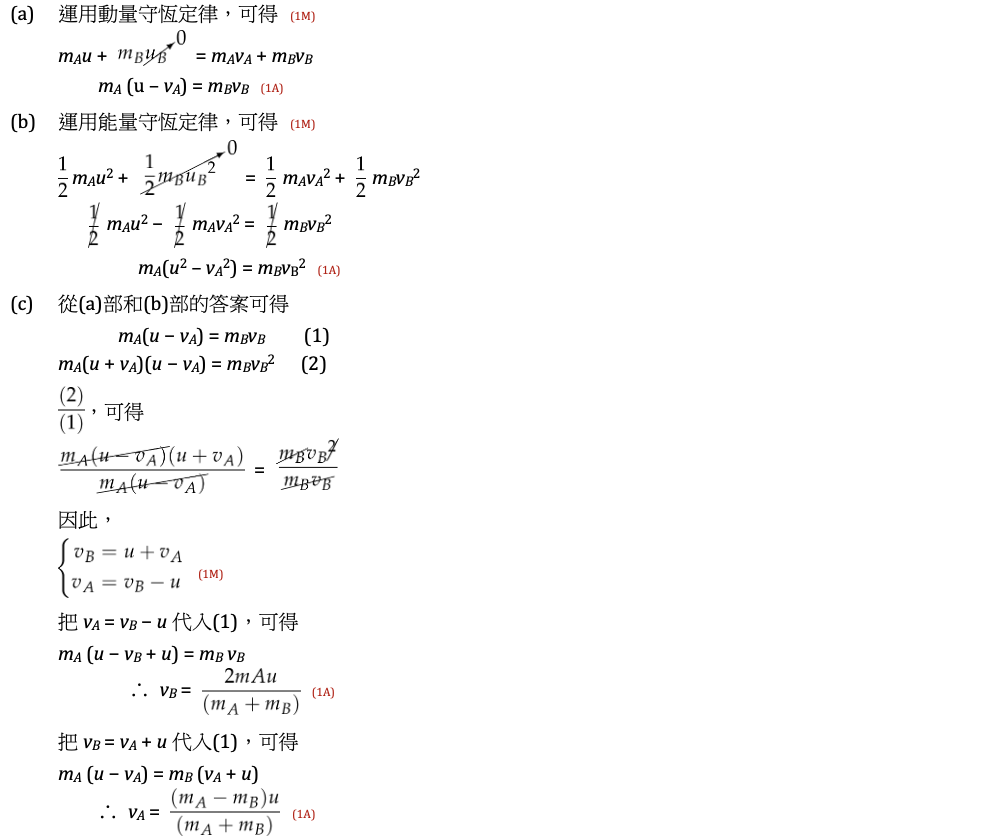
\includegraphics[width=\textwidth]{./img/ch5_momentum_lq_2024-05-11-22-45-13.png}\par}
}



\newprob{1715432917}
{
    % active  phys p289 *6
    把一根長度為$\ell$而質量為$M$的均勻木棒放在平滑 的水平面上。一顆質量為$m$ 的點質量以速率$v$趨 向木棒,最後跟木棒碰撞。碰撞後,點質量便停 下來。 \par 在以下情況中,木棒的重心碰撞後的速率是多 少?假設碰撞是彈性的。
    \par{\par\centering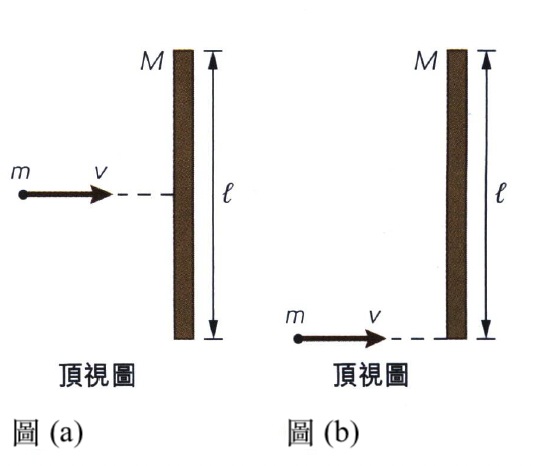
\includegraphics[width=.4\textwidth]{./img/ch5_momentum_lq_2024-05-11-21-10-19.png}\par}
    \begin{parts}
        \part 點質量擊中木棒的中心(圖a)。
        \part 點質量擊中木棒的一端(圖b)。木棒碰撞後 向右方移動並旋轉。
    \end{parts}
    \dlines{1}\clearpage\dlines{1}
}{
    \sol
    \par{\par\centering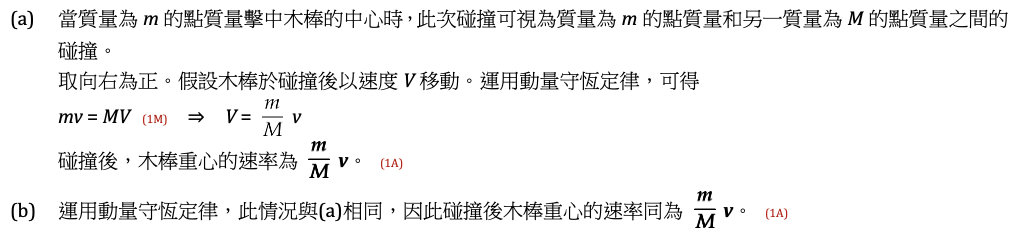
\includegraphics[width=\textwidth]{./img/ch5_momentum_lq_2024-05-11-22-45-54.png}\par}
}